\documentclass[ngerman,11pt,a4paper]{report}
\usepackage[utf8]{inputenc}
\usepackage{csquotes}
\usepackage{amsmath}
\usepackage{amsfonts}
\usepackage{amssymb}
\usepackage{dsfont}
\usepackage{algorithm}
\usepackage{algpseudocode}
\usepackage[dvipsnames]{xcolor}
\usepackage{pdfpages}
\usepackage{translator}
\usepackage{babel}
\usepackage{graphicx}
\usepackage{wrapfig}
\usepackage{color,soul}
\usepackage[bottom]{footmisc}
\usepackage{float}
\usepackage[section]{placeins}
\usepackage[backend=biber,style=numeric,sorting=none]{biblatex}
\usepackage[format=hang]{caption}
\usepackage{pgfgantt}
\usepackage[export]{adjustbox}
\usepackage{multicol}
\usepackage{xurl}
\usepackage{fancyhdr}
\usepackage{pgfkeys}
\usepackage[dvipsnames]{xcolor}
\usepackage{tikz}
\usepackage{tkz-euclide}
\usepackage{pgfplots}
\pgfplotsset{compat=1.18}
\usetikzlibrary{calc,positioning}
\usepackage{hyperref}
\usepackage[acronym,automake,nomain]{glossaries}

%---------------------------------------------------------------------------------------
\makeglossaries
\addbibresource{verweise.bib}

%PageLayout
\linespread{1.2}
\usepackage[top=2.7cm, bottom=2.8cm, left=3cm, right=3cm, headheight=20pt]{geometry}
\pagestyle{fancy}
\fancyhead{}
\fancyhead[R]{\footnotesize \fancyplain{}{\textit{\leftmark}}}
\fancyfoot{}
\fancyfoot[R]{Seite \thepage}
\fancypagestyle{plain}
{%
	\fancyhf{} % clear all header and footer fields
	\fancyfoot[R]{Seite \thepage} % except the center
	\renewcommand{\headrulewidth}{0pt}
}

%Defintions
\usepackage[framemethod=TikZ]{mdframed}
\newcounter{def}[chapter]\setcounter{def}{0}
\renewcommand{\thedef}{\arabic{chapter}.\arabic{def}}
\newenvironment{Definition}[2]
{
	\refstepcounter{def}
	\mdfsetup
	{
    	frametitle=
    	{
	        \tikz[baseline=(current bounding box.east),outer sep=0pt]
	        \node[anchor=east,rectangle,fill=Green!40]
	        {\strut Definition~\thedef:~#1};
	    },
	    innertopmargin=10pt,linecolor=Green!40,
    	linewidth=2pt,topline=true,
	    frametitleaboveskip=\dimexpr-\ht\strutbox\relax
	}
	\begin{mdframed}[backgroundcolor=Green!10]\relax
	\label{#2}
}
{
	\end{mdframed}
}

%Theorems
\newcounter{theo}[chapter]\setcounter{theo}{0}
\renewcommand{\thetheo}{\arabic{chapter}.\arabic{theo}}
\newenvironment{Satz}[2]
{
	\refstepcounter{theo}
	\mdfsetup
	{
    	frametitle=
    	{
	        \tikz[baseline=(current bounding box.east),outer sep=0pt]
	        \node[anchor=east,rectangle,fill=Green!40]
	        {\strut Satz~\thetheo:~#1};
	    },
	    innertopmargin=10pt,linecolor=Green!40,
    	linewidth=2pt,topline=true,
	    frametitleaboveskip=\dimexpr-\ht\strutbox\relax
	}
	\begin{mdframed}[backgroundcolor=Green!10]\relax
	\label{#2}
}
{
	\end{mdframed}
}

%Algorithms
\floatname{algorithm}{Algorithmus}
\renewcommand{\algorithmicrequire}{\textbf{Eingabe:}}
\renewcommand{\algorithmicensure}{\textbf{Ausgabe:}}
%---------------------------------------------------------------------------------------
%New commands
\newcommand{\argmin}{\mathop{\mathrm{arg\,min}}} 		% argmin
\newcommand{\p}{\par\bigskip\noindent}					% Für Absätze
\newcommand{\acrshortmath}[1]{\text{\acrshort{#1}}}		% Für Zugriff auf Glossary in Mathe-Umgebungen

%Math-Operator
\DeclareMathOperator{\sign}{sgn}


\author{Vipin Singh}
\title{BA_Thesis}
\date{\today}

\begin{document}
	
\includepdf{deckblatt}
    
    \begin{abstract}
    	\FloatBarrier %Verhindert Fehlpositionierung von Abbildungen aus vorherigen Abschnitten
	    \setcounter{page}{2}
	    \phantomsection
    	\addcontentsline{toc}{chapter}{Zusammenfassung}
    	Das Ziel der vorliegenden Arbeit ist es, Verfahren der Deflektometrie für spiegelnde und transparente Prüfoberflächen einzuführen und mathematisch zu erklären.
Der Fokus liegt darauf, mithilfe der Verfahren die Sichtprüfung für diese Oberflächen zu ermöglichen.
Dabei wird erklärt, welche Methoden im wissenschaftlichen Gebiet der Deflektometrie eingesetzt werden, um Oberflächen vollständig zu erfassen.
Zur Bearbeitung des Themas werden transparente Brillengläser und spiegelnde Keramikobjekte analysiert und mit den eingeführten Verfahren automatisiert ausgewertet.
Die Ergebnisse der Auswertung durch die eingeführten Verfahren zeigen, dass es möglich ist, Anomalien der Oberflächenkrümmung spiegelnder und transparenter Prüfobjekte, wie z. B. Pickel, Dellen, Kratzer oder Gravuren, zu erfassen.
Dadurch wird es ermöglicht, Oberflächendefekte spiegelnder und transparenter Prüfobjekte zu lokalisieren und qualitative Aussagen der Oberflächenbeschaffenheit zu formulieren.
    \end{abstract}
    
    %Inhaltsverzeichnis
    {
    	\FloatBarrier %Verhindert Fehlpositionierung von Abbildungen aus vorherigen Abschnitten
	    \setcounter{page}{3}
	    \phantomsection
	    \addcontentsline{toc}{chapter}{Inhaltsverzeichnis}
	    {%\small
	    	\tableofcontents
	    }
    }
    
    %Abbildungsverzeichnis
    {
	    \FloatBarrier %Verhindert Fehlpositionierung von Abbildungen aus vorherigen Abschnitten
    	\newpage
    	\phantomsection
    	\addcontentsline{toc}{chapter}{Abbildungsverzeichnis}
    	\listoffigures
    }
    
    %Abkürzungsverzeichnis
    {
    	\FloatBarrier %Verhindert Fehlpositionierung von Abbildungen aus vorherigen Abschnitten
			\newpage        
			\phantomsection
			\addcontentsline{toc}{chapter}{Abkürzungsverzeichnis}
			\printglossary[title=Abkürzungsverzeichnis, type=\acronymtype]
			\newacronym{lr}{$l_r$}{Deflektometrische Registrierung}
\newacronym{lwidth}{$L_{width}$}{Breite des Monitorbildes in Pixel}
\newacronym{lheight}{$L_{height}$}{Höhe des Monitorbildes in Pixel}
\newacronym{lrx}{$l_{r,x}$}{Deflektometrische Registrierung der Spaltenpositionen}
\newacronym{lry}{$l_{r,y}$}{Deflektometrische Registrierung der Zeilenpositionen}
\newacronym{d}{$D$}{Definitionsmenge}
    }
    
    %Einführung
    {
    	\FloatBarrier %Verhindert Fehlpositionierung von Abbildungen aus vorherigen Abschnitten
    	\chapter{Einführung}
      \label{chp:einfuehrung}
      Durch die optischen Besonderheiten von spiegelnd glänzenden Oberflächen treten solche in der Industrie an vielen Stellen auf.
Speziell in der Automobilindustrie werden täglich große Karosserieflächen glänzend lackiert.
Alleine in Deutschland wurden in den Jahren von 1990 bis 2021 im Durchschnitt ungefähr 5 Millionen Personenkraftwagen pro Jahr produziert \cite{statistaPKW}.
Ein großer Teil der Fahrzeuge erhalten nach der Lackierung eine spiegelnde Oberfläche.
Solche Oberflächen müssen durch besondere Verfahren auf Defekte überprüft werden.
Dabei sorgen spekulare Reflexionen dafür, dass die Oberflächen nicht direkt, sondern über ihre Spiegelbilder der Umgebung betrachtet werden müssen. %TODO Beispielbilder?

\p
Die riesige Menge an Oberflächen macht es für die Qualitätssicherung unumgänglich die Prüfung durch automatisierte Prozesse zu integrieren.
Dabei stoßen die üblichen Verfahren der industriellen Bildverarbeitung auf ihre Grenzen, sodass neue Methoden eingeführt werden müssen.
Diese speziellen Anwendungen erfordern den Einsatz von deflektometrischen Prüfaufbauten.
In der Industrie sind solche Verfahren schon seit Längerem zur Analyse der Topographie von spiegelnden Freiformflächen etabliert.
Deflektometrische Verfahren funktionieren nach einem ähnlichen Prinzip, wie auch die Inspektion von spiegelnden Oberflächen durch Menschen. %TODO Ergänzen wie das Prinzip der Menschen funktioniert.
Das wissenschaftliche Gebiet der Deflektometrie ist auch heute noch Thema für viele Forschungsarbeiten und wird stetig weiterentwickelt.

\p
Im Rahmen der Arbeit werden spekular reflektierende Objektoberflächen unter Projektion von bekannten Mustern durch eine Kamera aufgenommen, anschließend analysiert und auf Defekte überprüft.
Welche Informationen können aus der Beobachtung von Spiegelbildern gewonnen werden?
Wie sehen allgemein anwendbare Methoden aus, um spiegelnde Oberflächen erfolgreich zu bewerten?
Das Ziel der Arbeit ist es, diese Fragen zu erforschen und aufzuklären.
Des Weiteren sollen ein Aufbau, die Ansteuerung von Beleuchtung und Kamera und die notwendige Auswertung des Bildmaterials entwickelt werden, durch welche eine Erkennung von Oberflächendefekten ermöglicht wird.
Die Umsetzung soll dabei in Form einer Softwareerweiterung für NeuroCheck erfolgen, eines sogenannten \textit{Plug-ins}.

\p
Während der Arbeit soll außerdem ein bestimmter Sonderfall genauer betrachtet werden - transparente Prüfobjekte.
Die Problematik ist dabei, dass man neben der Reflexion des Lichts, mit der Transmission zu kämpfen hat.
Dafür gibt es verschiedene Lösungsansätze wie z. B. die Auftragung einer undurchsichtigen Beschichtung.
Eine andere Möglichkeit ist eine Veränderung in dem Prüfaufbau.
Anstatt ein Muster auf das Objekt zu projizieren, kann man eine Durchlichtbeleuchtung nutzen.
Das heißt, dass man auf einem Bildschirm unter dem transparenten Prüfobjekt verschiedene Muster anzeigt.

\p
Durch die aufgenommenen Muster können Aussagen über die Oberflächenbeschaffenheit getroffen werden.
Abhängig von den verwendeten Mustern und der Auswertung sollen damit bestimmte Fehlstellen kenntlich gemacht werden.
Als Fehlstellen gelten Verformungen und Oberflächendefekte wie z. B. Dellen, Kratzer oder matte Stellen.
%TODO Weiteres schreiben im Bezug auf die nachfolgende Arbeit (vermutlich eher gegen Ende)
%Zur Detektion dieser Defekte kann man verschiedene deflektometrische Verfahren einsetzen.
%Die Verfahren können verschiedene Ergebnisse liefern, abhängig davon sind eventuell aus den Ergebnissen weitere Verarbeitungen und Auswertungen nötig.
%Im Rahmen des Projektes werden speziell die deflektometrischen Verfahren betrachtet, welche für eine Vielzahl von Anwendungen genutzt werden können.
%Nachfolgende Verarbeitungen, z. B. Detektion von Zeichen und Kratzern, werden im Rahmen des Projekts und der Bachelor-Arbeit nicht genauer behandelt.
    }
    
    %Sichtprüfung durch Lichtreflexionen
    {
    	\FloatBarrier %Verhindert Fehlpositionierung von Abbildungen aus vorherigen Abschnitten
    	\chapter{Sichtprüfung durch Lichtreflexionen}
    	%Prüfaufbau
{
	\FloatBarrier
    \section{Prüfaufbau}
    \label{sec:pruefaufbau}
    Die folgende Abbildung soll eine Skizze des verwendeten Prüfaufbaus zeigen.
Die Skizze ist zur Vereinfachung ohne Halterungen erstellt worden.

\begin{figure}[H]
	\centering
	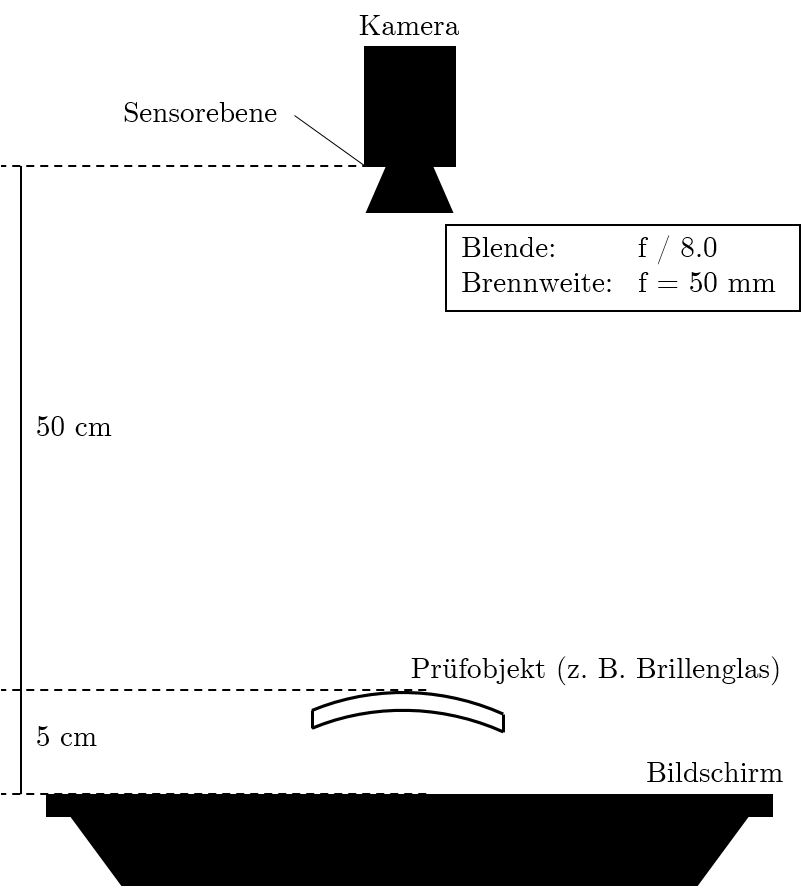
\includegraphics[width=0.5\textwidth]{03_sichtpruefungDurchLichtreflexionen/pruefaufbau/figures/aufbau}
	\caption[Prüfaufbau]{Prüfaufbau (Abbildung nicht maßstabsgetreu)}
	\label{img:prüfaufbau}
\end{figure}

\noindent
Die Parameter des Prüfaufbaus wie z. B. Kameraeinstellungen und Entfernungen lassen sich aus Abbildung \ref{img:prüfaufbau} entnehmen.
Es gilt zu beachten, dass die Entfernung zur Kamera nicht am Objektiv, sondern an der Sensorebene gemessen wird.
Der Grund liegt darin, dass Objektive keine festgelegte Größe haben, weshalb die Entfernung andernfalls für verschiedene Objektive unterschiedlich sein würde.
Die Sensorebene einer Kamera ist die Position des Kamerasensors, an der das einfallende Licht aufgenommen wird.
Dieser Aufbau wird zur Erzeugung von Bildmaterial für diesen Projektbericht verwendet.
Zur Auswertung und Verknüpfung des Bildmaterials wird die NeuroCheck-Software eingesetzt.
Die Prüfobjekte sind transparente Brillengläser mit Eingravierungen und einzelnen Fehlstellen.
}

%Verfahren
{
	\FloatBarrier
    \section{Verfahren}
    \label{sec:verfahren}
    Der erste Prototyp soll es ermöglichen, Kratzer und ähnliche Defekte auf transparenten Objekten mittels der Deflektometrie sichtbar zu machen.
Der Ansatz zur Erkennung basiert auf der Idee aus Abbildung \ref{img:scratch}.
Dabei nutzt man die abweichende Lichtreflexion an Kratzern und Defekten im Vergleich zur idealen spiegelnden Oberfläche des Objekts.

\begin{figure}[H]
	\centering
	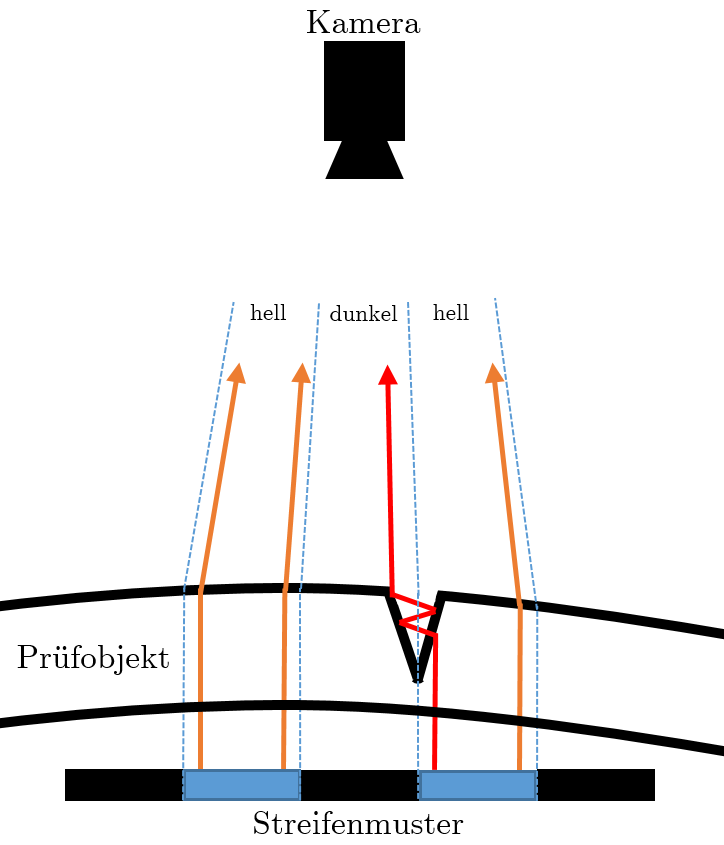
\includegraphics[width=0.5\textwidth]{03_sichtpruefungDurchLichtreflexionen/verfahren/figures/scratch_reflection}
	\caption[Lichtbrechung an einem Kratzer]{Lichtbrechung an einem Kratzer (Abbildung nicht maßstabsgetreu)}
	\label{img:lightreflection}
\end{figure}

\noindent
In Abbildung \ref{img:lightreflection} wird schematisch die Überlegung hinter dem Ansatz dargestellt.
Man nimmt ein Streifenmuster und projiziert dieses auf ein spiegelndes Prüfobjekt.
Für ein transparentes Prüfobjekt kann man das Streifenmuster als Durchlichtbeleuchtung von unten projizieren.
An den Hell-Dunkelübergän\-gen fällt Licht vom hellen Streifen in den Kratzer.
Durch den Kratzer werden manche Lichtstrahlen so reflektiert, dass diese an der Stelle des dunklen Streifens in die Kamera gelangen.
Dadurch erkennt man im Kamerabild eine lokale Fehlstelle, da der Kratzer heller ist als der umliegende dunkle Streifen.
Analog dazu erkennt man im hellen Streifen lokal eine etwas dunklere Stelle.
Durch Anpassung der Kameraeinstellungen kann man beeinflussen, wie stark man den Kratzer sieht.
Z. B. kann dies durch die Erhöhung der Belichtungszeit oder weitere Öffnung der Blende geschehen.
Dadurch wird ein Oberflächendefekt im dunklen Streifen zwar besser und stärker sichtbar, allerdings verliert man die Informationen über den Defekt im hellen Streifen.
Dies liegt daran, dass auch die dunklere Stelle im hellen Streifen so hell werden kann, dass sie nicht mehr von dem hellen Streifen selbst zu unterscheiden ist.
Dieses Problem erkennt man in der Abbildung \ref{img:scratches}.

\begin{figure}[H]
	\centering
	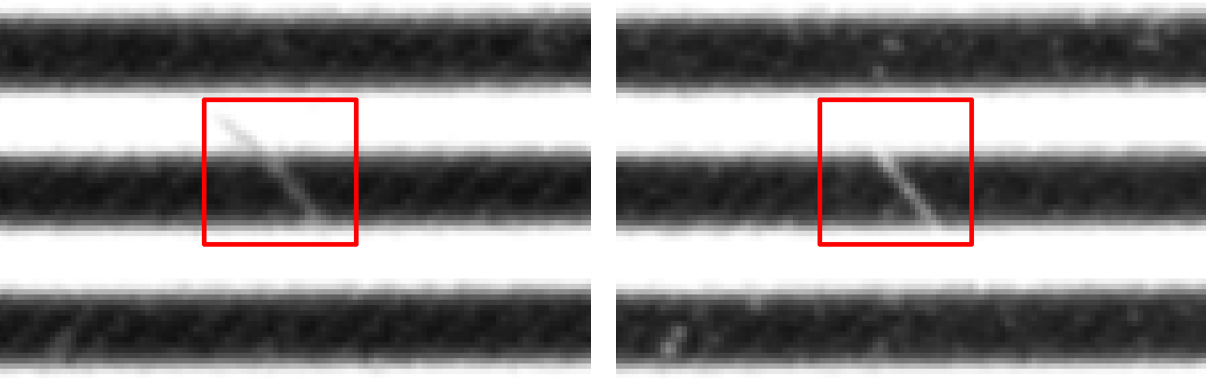
\includegraphics[width=\textwidth]{03_sichtpruefungDurchLichtreflexionen/verfahren/figures/visibleScratch}
	\caption[Kratzer]{Kratzer an Hell-Dunkel-Übergang. Links mit weniger weit geöffneten Blende im Vergleich zu rechts.}
	\label{img:scratches}
\end{figure}

\noindent
Trotz der fehlenden Information hat das rechte Bild den Vorteil, dass durch die größere Differenz zwischen dem Oberflächendefekt und dem Hintergrund eine bessere Erkennung möglich ist.
Das Problem mit unsichtbaren Teilen der Defekte ist aber nicht nur abhängig von der Kameraeinstellung, sondern auch von dem Oberflächendefekt selbst.

\begin{figure}[H]
	\centering
	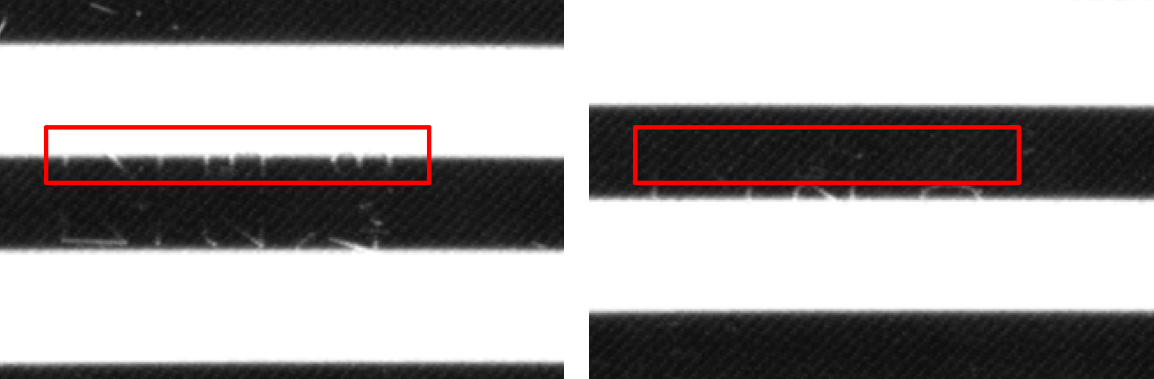
\includegraphics[width=\textwidth]{03_sichtpruefungDurchLichtreflexionen/verfahren/figures/minorScratch}
	\caption[Eingravierung im Glas]{Schlecht erkennbare Eingravierung im Glas, nach Verschiebung des Streifenmusters.}
	\label{img:engraving}
\end{figure}

\noindent
In Abbildung \ref{img:engraving} stellt man fest, dass besonders kleine Defekte der Oberflächenstruktur wie hier z. B. die Eingravierung nur zum Teil und auch nur in der Nähe der Übergänge zu erkennen sind.

\p
Daraus lassen sich bestimmte Folgerungen ziehen.
Zunächst decken Streifenmuster nur unmittelbar an den Übergängen zuverlässig Defekte auf.
Das bedeutet, um Defekte an bestimmten Stellen zu erfassen, muss das verwendete Streifenmuster an den Stellen Übergän\-ge haben.
So kann man schließen, dass Muster mit schmaleren Streifen besser geeignet sind, um auch kleinere Oberflächendefekte sichtbar zu machen.
Allerdings führt dies auch dazu, dass stets nur kleine Teile der Defekte zu erkennen sind.
Als Lösung dieses Problems kann man mehrere Streifenmuster verwenden, deren Streifen stets in ihrer Ausbreitungsrichtung verschoben sind.
Verknüpft man die sichtbaren Teile der Defekte, kann man ein vollständiges Gesamtbild erhalten.
In diesem Gesamtbild sollten alle Oberflächendefekte ab einer bestimmten Mindesttiefe sichtbar werden.
Die Mindesttiefe hängt dabei von den Kameraeinstellungen, der Beleuchtungsstärke und den verwendeten Streifenmustern ab.
}
    }
    
    %Deflektometrische Registrierung
    {
    	\FloatBarrier %Verhindert Fehlpositionierung von Abbildungen aus vorherigen Abschnitten
    	\chapter{Deflektometrische Registrierung}
    	\begin{Definition}{Deflektometrische Registrierung}{def:deflektometrischeRegistrierung}
	Die \textit{deflektometrische Registrierung} \acrshort{lr} beschreibt die Abbildung von Bildpunkten zu Schirmpunkten. \cite{kit_werling}
	%
	\begin{equation*}
		\acrshortmath{lr} : A_{Cam} \rightarrow L \cup \varnothing ,\quad P_{B} \rightarrow P_{L}
	\end{equation*}
	%
	$ A_{Cam} \subset \mathbb{R}^{2} $ bezeichnet die Menge der Bildpunkte bzw. der Kamerapixel.
	$ L \subset \mathbb{R}^{2} $ bezeichnet die Menge der Schirmpunkte bzw. der Monitorpixel.
	In Koordinatenschreibweise lässt sich die Abbildung somit darstellen als:
	%
	\begin{equation*}\label{eq:deflektometrischeRegistrierungAbbildung}
		\acrshortmath{lr} : \mathbb{R}^{2} \supset A_{Cam} \rightarrow \mathbb{R}^2 ,\quad (x_{B}, y_{B}) \mapsto (x_{L}, y_{L})
	\end{equation*}
\end{Definition}

\begin{Satz}{Separierbarkeit der deflektometrischen Registrierung}{theo:separierbarkeitDeflektometrischeRegistrierung}
Ferner kann die \textit{deflektometrische Registrierung} \acrshort{lr} in zwei Abbildungen von Bildpunkten zu den Spalten- und Zeilenpositionen der Schirmpunkte separiert werden:
	%
	\begin{equation*}
		\acrshortmath{lrx} : \mathbb{R}^{2} \supset A_{Cam} \rightarrow \mathbb{R} ,\quad (x_{B}, y_{B}) \mapsto x_{L}
	\end{equation*}
	%
	\begin{equation*}
		\acrshortmath{lry} : \mathbb{R}^{2} \supset A_{Cam} \rightarrow \mathbb{R} ,\quad (x_{B}, y_{B}) \mapsto y_{L}
	\end{equation*}
	%
\end{Satz}

\noindent
Die deflektometrische Registrierung kann aus der Beobachtung des Monitors mithilfe der Kamera aufgestellt werden.
Wird der Monitor indirekt über eine spiegelnde Oberfläche beobachtet, können aus der deflektometrischen Registrierung Krümmungsmerkmale über die spiegelnde Oberfläche bestimmt werden.
Durch die Berücksichtigung der Positionen der Systemkomponenten können mittels der deflektometrischen Registrierung Höheninformationen über die Oberfläche gewonnen werden.
Dieses Verfahren wurde im Abschnitt \ref{sub:rekonstruktion} bereits beschrieben.

%Bestimmung der deflektometrischen Registrierung
{
	\FloatBarrier
    \section{Bestimmung der deflektometrischen Registrierung}
    \label{sec:bestimmungDeflektometrischeRegistrierung}
    Die Bestimmung der deflektometrischen Registrierung nach Definition \ref{def:deflektometrischeRegistrierung} bedeutet eine Zuordnung von Kamerapixeln zu Monitorpixeln.
Grundsätzlich soll jeder Lichtstrahl, der über das Prüfobjekt in die Kamera reflektiert wird im Kamerabild identifizierbar sein.
Eine einfache Möglichkeit eine solche Zuordnung zu erreichen bekommt man, indem man die Pixel des Monitors einzeln einschaltet und dabei die Veränderung im Kamerabild betrachtet.
Bei kleinen Bildern ist dies noch umsetzbar, allerdings wird die Anzahl von Pixeln mit zunehmender Auflösung schnell sehr groß und unübersichtlich, sodass dieser Ansatz nicht praktikabel ist.
Aus dem Grund ist es effektiver Bilder auf dem Monitor anzuzeigen, die Positionen visuell codieren können.
Durch die visuelle Erfassung des Spiegelbilds können somit die zugehörigen Positionen auf dem Monitor berechnet werden.

\p
Ein herkömmliches Kodierverfahren für solche Prozesse ist das Phasenschiebeverfahren.
Der Ansatz bei dem Verfahren ist es die Zeilen- und Spaltenpositionen des Monitors durch periodische Muster zu kodieren.
Die Grauwerte von periodischen Mustern nehmen dabei Werte an, die über die periodische Funktion bestimmt wurden.
Die hier verwendeten Funktionen sind Kosinusfunktionen.
Damit können die Pixel des Musters Phaseninformationen eines lokalen Orts übertragen.
Durch die Periodizität der Funktionen kann aus der reinen Phaseninformation noch nicht die genaue Monitorposition bestimmt werden.
Die Lösung dieses Problems wird als Phasenentfaltung bezeichnet (siehe auch Definition \ref{def:phasenentfaltung}).
Hierzu stellt Werling in seiner Arbeit \cite{kit_sbw} ein mehrstufiges Phasenschiebeverfahren vor, das Muster mit unterschiedlichen Perioden verwendet.

\begin{Definition}{Phasenentfaltung}{def:phasenentfaltung}
	Die \textit{Phasenentfaltung} bezeichnet den Vorgang zur Auflösung der mehrdeutigen Zuordnung der Phaseninformation.
\end{Definition}

%Deflektometrische Registrierung ohne Phasenentfaltung
{
	\FloatBarrier
    \subsection{Deflektometrische Registrierung ohne Phasenentfaltung}
    \label{sub:registrierungOhnePhasenentfaltung}
    Ohne eine Phasenentfaltung bekommt man eventuell eine mehrdeutige Zuordnung aufgrund der Periodizität der Kosinusfunktion.
Soll eine eindeutige Zuordnung über das Phasenschiebeverfahren ohne Phasenentfaltung erfolgen, darf es also nur eine einzige Musterperiode auf der Monitorbreite bzw. Monitorhöhe geben.
Damit lässt sich die Kodierung der Monitorkoordinaten $(x_{L}, y_{L})$ durch die Phasen $(\phi_{x}, \phi_{y})$ folgendermaßen aufstellen:
%
\begin{equation}\label{eq:phasenkodierung}
	x_{L} = \dfrac{\text{\acrshort{lwidth}}}{2\pi}\phi_{x},
	\qquad
	y_{L} = \dfrac{\text{\acrshort{lheight}}}{2\pi}\phi_{y}
\end{equation}
%
\noindent
Die Monitorbreite wird dabei mit \acrshort{lwidth} und die Monitorhöhe mit \acrshort{lheight} angegeben.

\p
O.B.d.A. wird nachfolgend nur die deflektometrische Registrierung der Spaltenpositionen \acrshort{lrx} ($x$-Richtung) betrachtet.
Die deflektometrische Registrierung der Zeilenpositionen \acrshort{lry} ($y$-Richtung) kann analog bestimmt werden.
Das $k$-te Muster $m_k$ zur Kodierung der Monitorpunkte wird durch eine Kosinusfunktion aufgebaut und hat die Form:
%
\begin{equation}\label{eq:monitormuster}
	\begin{split}	
		m_k(x_L,y_L) = A_m \left(1 + C_m \cos \left(\dfrac{2\pi}{\text{\acrshort{lwidth}}} x_L + \psi_k\right)\right),
		\qquad
		k \in \lbrace 1,\ldots,N_{shift}\rbrace, \\
		\psi_k = (k - 1)\dfrac{2\pi}{N_{shift}}
	\end{split}
\end{equation}
%
$A_m$ bezeichnet die Amplitude, $C_m$ den Kontrast, $\psi_k$ die Phasenverschiebung des $k$-ten Musters und $N_{shift}$ die Anzahl an Mustern für das Phasenschiebeverfahren.
Das Muster wird auf dem Monitor angezeigt und über eine spiegelnde Oberfläche durch die Kamera beobachtet.
Über die Reflexion an der Oberfläche trifft der Sichtstrahl ausgehend vom Bildpunkt $(x_B, y_B)^\top \in A_{Cam}$ den Monitor im Punkt $(x_L, y_L)^\top \in L \cup \varnothing$ bestimmt durch die Abbildung aus der Gleichung \ref{eq:deflektometrischeRegistrierungAbbildung}:
%
\begin{equation}
	\begin{pmatrix}
		x_L \\ 
		y_L
	\end{pmatrix}
	= \text{\acrshort{lr}}(x_B, y_B) = 
	\begin{pmatrix}
		\text{\acrshort{lrx}}(x_B, y_B) \\ 
		\text{\acrshort{lry}}(x_B, y_B)
	\end{pmatrix} 
\end{equation}
%
Dementsprechend lässt sich das $k$-te Kamerabild $g$ am Bildpunkt $(x_B, y_B)^\top$ beschreiben durch das $k$-te Muster am Punkt $\text{\acrshort{lrx}}(x_B, y_B), \text{\acrshort{lry}}(x_B, y_B))^\top$:
%
\begin{equation}
	g_k(x_B, y_B) = m_k(\text{\acrshort{lrx}}(x_B, y_B), \text{\acrshort{lry}}(x_B, y_B))
\end{equation}
%
Setzt man für $m_k$ die Gleichung \ref{eq:monitormuster} unter Berücksichtigung der Veränderung durch die Oberfläche erhält man:
%
\begin{equation}\label{eq:kamerabild}
	g_k(x_B, y_B) = A_g(x_B, y_B) \left(1 + C_g(x_B, y_B) \cos \left(\dfrac{2\pi}{\text{\acrshort{lwidth}}}\text{\acrshort{lrx}}(x_B, y_B) + \psi_k\right)\right)
\end{equation}
%
Dabei sind die Amplitude $A_g$ und der Kontrast $C_g$ des Musters im Kamerabild unter Umständen unterschiedlich zu dem angezeigten Muster im Monitorbild.
Der Unterschied ist abhängig von dem Oberflächenpunkt an dem der Sichtstrahl reflektiert wird.
Aus dem Grund werden $A_g$ und $C_g$ in Abhängigkeit vom Kamerabildpunkt $(x_B, y_B)^\top$ angegeben.

\p
Durch Umstellung der Gleichung \ref{eq:phasenkodierung} nach der Phase und Einsetzen der deflektometrischen Registrierung \acrshort{lr}, erhält man die Phase $\phi_x$ des $k$-ten Musters in Abhängigkeit von den Kamerabildpunkten:
%
\begin{equation}\label{eq:phaseBildkoordinaten}
	\phi_x = \dfrac{2\pi}{\text{\acrshort{lwidth}}}\text{\acrshort{lrx}}(x_B, y_B)
\end{equation}
%
Durch Einsetzen der Phase aus Gleichung \ref{eq:phaseBildkoordinaten} in die Gleichung \ref{eq:kamerabild} des Kamerabilds erhält man den Zusammenhang zwischen der Phase $\phi_x$ des $k$-ten Musters und dem Kamerabild   $g_k$:
%
\begin{equation}\label{eq:kamerabildMitPhase}
	g_k(x_B, y_B) = A_g(x_B, y_B) \left(1 + C_g(x_B, y_B) \cos \left(\phi_x(x_B, y_B) + \psi_k\right)\right)
\end{equation}
%
Unter Einbeziehung der $N_{shift}$-vielen phasenverschobenen Streifenmuster kann man die Phase $\phi_x$ berechnen:
%
\begin{equation}\label{eq:tanPhase}
	\tan (\phi_x) = -\dfrac{\sum\limits_{k=1}^{N_{shift}} g_k(x_B, y_B) sin(\psi_k)}{\sum\limits_{k=1}^{N_{shift}} g_k(x_B, y_B) cos(\psi_k)}
\end{equation}
%
Aus den Gleichungen \ref{eq:phasenkodierung} und \ref{eq:tanPhase} folgt schließlich:
%
\begin{equation}\label{eq:registrierungX}
	x_L = \text{\acrshort{lrx}}(x_B, y_B) = 
	\dfrac{\text{\acrshort{lwidth}}}{2\pi}
	\arctan 
	\left( 
		-\dfrac
		{\sum\limits_{k=1}^{N_{shift}} g_k(x_B, y_B) sin\left((k - 1)\dfrac{2\pi}{N_{shift}}\right)}
		{\sum\limits_{k=1}^{N_{shift}} g_k(x_B, y_B) cos\left((k - 1)\dfrac{2\pi}{N_{shift}}\right)}
	\right)
\end{equation}
%
Mittels der Gleichung \ref{eq:registrierungX} ist somit die deflektometrische Registrierung in $x$-Richtung angegeben und die Monitorpositionen eindeutig bestimmt.
Die deflektometrische Registrierung in $y$-Richtung lässt sich analog dazu bestimmen.
Die Anzahl an Mustern bzw. Phasenverschiebungen $N_{shift}$ ist noch als Parameter übrig geblieben.
Um eine eindeutige Zuordnung zu erhalten, benötigt man aufgrund der drei unbekannten Größen Amplitude $A_g$, Kontrast $C_g$ und Phase $\phi_x$ in Gleichung \ref{eq:kamerabildMitPhase} eine Mindestanzahl von drei Phasenverschiebungen.

\p
Durch die Eindeutigkeit der Phase in dem verwendeten Muster spart man sich die Phasenentfaltung.
Dennoch ist das Phasenschiebeverfahren nach diesem Ansatz nicht sehr präzise und daher eher ungeeignet für Praxisanwendungen.
Der Grund liegt darin, dass Monitore lediglich eine vergleichsweise kleine Anzahl an Helligkeitsstufen darstellen können.
Die Anzahl an zu kodierenden Pixelpositionen sind in der Regel deutlich größer.
Eine ähnliche Beschränkung gibt es auch bei der Bildaufnahme, denn auch die Kamera nimmt eine Quantisierung vor und kann nicht sämtliche Helligkeitsstufen aufnehmen.
Zusammengenommen ist die Auflösung der Monitorpunkte damit stark begrenzt.
Eine höhere Ortsauflösung lässt sich erreichen indem man Muster mit mehreren Perioden über die Monitorbreite bzw. Monitorhöhe verwendet.
Damit wird schließlich eine Phasenentfaltung als zusätzliche Aufgabe erforderlich.
}
}

%Auswertung der deflektometrischen Registrierung
{
	\FloatBarrier
    \section{Auswertung der deflektometrischen Registrierung}
    \label{sec:auswertungDeflektometrischeRegistrierung}
    Die deflektometrische Registrierung \acrshort{lr} kann nicht ohne Weiteres direkt ausgewertet werden.
Deshalb wird im Folgenden die Weiterverarbeitung der deflektometrischen Registrierung beschrieben, sodass bekannte Methoden aus dem Gebiet der Bildverarbeitung angewendet werden können.

\p
Die graphische Darstellung der deflektometrischen Registrierung \acrshort{lr} stellt sich zunächst als schwierig heraus, da man mit einer Abbildung der Form $\acrshortmath{real}^2 \rightarrow \acrshortmath{real}^2$ arbeitet.
Aus dem Grund wird die Separierbarkeit der deflektometrischen Registrierung aus Satz \ref{theo:separierbarkeitDeflektometrischeRegistrierung} angewendet.
Daraus erhält man die beiden Abbildungen der Form $\acrshortmath{real}^2 \rightarrow \acrshortmath{real}$:
%
\begin{equation*}
	\acrshortmath{lrx} : \acrshortmath{real}^{2} \supset A_{Cam} \rightarrow \acrshortmath{real} ,\quad (x_{B}, y_{B}) \mapsto x_{L}
\end{equation*}
%
\begin{equation*}
	\acrshortmath{lry} : \acrshortmath{real}^{2} \supset A_{Cam} \rightarrow \acrshortmath{real} ,\quad (x_{B}, y_{B}) \mapsto y_{L}
\end{equation*}
%
In der Form lässt sich die Analogie zu der mathematischen Beschreibung eines Graubildes $f$ erkennen:
%
\begin{equation*}
	f : \acrshortmath{real}^{2} \supseteq [x_{min},x_{max}] \times [y_{min},y_{max}] \rightarrow [I_{min},I_{max}] \subseteq \acrshortmath{real} ,\quad (x,y) \mapsto f(x,y)
\end{equation*}
%
Für die Darstellung als Bilder sind somit lediglich geeignete Transformationen der Wertemengen der deflektometrischen Registrierungen \acrshort{lrx} und \acrshort{lry} nötig.
%
\begin{Definition}{Darstellung der Deflektometrischen Registrierung}{def:graphDeflektometrischeRegistrierung}
	Die deflektometrischen Registrierung \acrshort{lr} kann als zwei einzelne Graubilder \acrshort{frx} und \acrshort{fry} dargestellt werden.
	%	
	\begin{equation*}
		\acrshortmath{frx} : \acrshortmath{real}^2 \supset \acrshortmath{d}(\acrshortmath{lrx}) \rightarrow [I_{min},I_{max}] \subseteq \acrshortmath{real}
	\end{equation*}
	%
	\begin{equation*}
		\acrshortmath{fry} : \acrshortmath{real}^2 \supset \acrshortmath{d}(\acrshortmath{lry}) \rightarrow [I_{min},I_{max}] \subseteq \acrshortmath{real}
	\end{equation*}
	%
	Die Bilder \acrshort{frx} und \acrshort{fry} sind definiert durch:
	%	
	\begin{equation*}
		\acrshortmath{frx}(x,y) := t_x(\acrshortmath{lrx}(x,y))
	\end{equation*}
	%	
	\begin{equation*}
		\acrshortmath{fry}(x,y) := t_y(\acrshortmath{lry}(x,y))
	\end{equation*}
	%
	Mit $\acrshortmath{d}(\acrshortmath{frx}) = \acrshortmath{d}(\acrshortmath{lrx})$ und $\acrshortmath{d}(\acrshortmath{fry}) = \acrshortmath{d}(\acrshortmath{lry})$ und
	%
	\begin{equation*}
		t_x : \acrshortmath{real} \supset \acrshortmath{w}(\acrshortmath{lry}) \rightarrow [I_{min},I_{max}] \subseteq \acrshortmath{real}
	\end{equation*}
	%
	\begin{equation*}
		t_y : \acrshortmath{real} \supset \acrshortmath{w}(\acrshortmath{lry}) \rightarrow [I_{min},I_{max}] \subseteq \acrshortmath{real}
	\end{equation*}
	%
	Die Transformationen $t_x$ und $t_y$ sind definiert als:
	%	
	\begin{equation*}
		t_x(x) := \left(\dfrac{x}{\acrshortmath{lwidth}}(I_{max} - I_{min})\right) + I_{min}
	\end{equation*}
	%	
	\begin{equation*}
		t_y(y) := \left(\dfrac{y}{\acrshortmath{lheight}}(I_{max} - I_{min})\right) + I_{min}
	\end{equation*}
	%
\end{Definition}
%
Die Abbildungen $t_x$ und $t_y$ sind dabei lineare Transformationen der Wertemengen der deflektometrischen Abbildungen in Spalten und Zeilen zu den zulässigen Intensitäten für die Bilder \acrshort{frx} und \acrshort{fry}, angegeben durch das Intervall $[I_{min},I_{max}]$.

\p
Erstellt man aus der berechneten deflektometrischen Registrierung \acrshort{lr} einer ungekrümmten Fläche die zugehörigen Bilder \acrshort{frx} und \acrshort{fry} nach Definition \ref{def:graphDeflektometrischeRegistrierung}, erhält man Darstellungen wie in Abbildung \ref{tikz:abbOptimaleSpaltenZeilenReg}:

% Abbildung: Optimale Spalten- und Zeilenregistrierung
{
	\begin{figure}[H]
		\centering
		\begin{adjustbox}{width=\textwidth}
	\begin{tikzpicture}[every node/.style={inner sep=0,outer sep=0}]
	
		\node [anchor=north west] (imgSpalten) at (0,0) {
\includegraphics[width=.47\textwidth]{04_deflektometrischeRegistrierung/auswertungDeflektometrischeRegistrierung/figures/spaltenRegistrierung_optimal}};
		\node [below=0.2cm of imgSpalten] {Graubild der Spaltenzuordnung \acrshort{frx}$(x,y)$};
		\node [anchor=north west] (imgZeilen) at (0.53\textwidth,0) {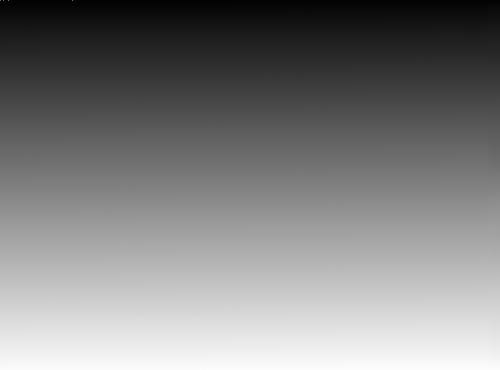
\includegraphics[width=.47\textwidth]{04_deflektometrischeRegistrierung/auswertungDeflektometrischeRegistrierung/figures/zeilenRegistrierung_optimal}};
		\node [below=0.2cm of imgZeilen] {Graubild der Zeilenzuordnung \acrshort{fry}$(x,y)$};
	
	\end{tikzpicture}
\end{adjustbox}
\caption[Darstellung Spalten- und Zeilenregistrierung]{Darstellung der Spalten- und Zeilenregistrierung als Bilder in Graustufen mit $I_{min} = 0$ und $I_{max} = 255$. Je dunkler ein Pixel ist, desto weiter links bzw. oben befindet sich die zugeordnete Spalten- bzw. Zeilenposition.}
		\label{tikz:abbOptimaleSpaltenZeilenReg}
	\end{figure}
}

\noindent
In Abbildung \ref{tikz:abbOptimaleSpaltenZeilenReg} wird direkt das Muster auf dem Monitor betrachtet.
Aus dem Grund lässt sich erkennen, dass die Zuordnung von Monitor- und Kamerapixeln in den Spalten und Zeilen linear verläuft.
Werden nun die Streifen durch besondere Oberflächeneigenschaften gekrümmt oder verzerrt, dann werden an diesen Stellen in den Bildern der deflektometrischen Registrierung Abweichungen vom linearen Grauwerteverlauf sichtbar.

% Abbildung: Brillenglas Registrierung
{
	\begin{figure}[H]
		\centering
		\begin{adjustbox}{width=\textwidth}
	\begin{tikzpicture}[every node/.style={inner sep=0,outer sep=0}]
	
		\node [anchor=north west] (imgSpalten) at (0,0) {\includegraphics[width=.47\textwidth]{04_deflektometrischeRegistrierung/auswertungDeflektometrischeRegistrierung/figures/streifenKrümmung_spalten}};
		\node [below=0.2cm of imgSpalten] {Graubild der Spaltenzuordnung \acrshort{frx}$(x,y)$};
		\node [anchor=north west] (imgZeilen) at (0.53\textwidth,0) {\includegraphics[width=.47\textwidth]{04_deflektometrischeRegistrierung/auswertungDeflektometrischeRegistrierung/figures/streifenKrümmung_zeilen}};
		\node [below=0.2cm of imgZeilen] {Graubild der Zeilenzuordnung \acrshort{fry}$(x,y)$};
	
	\end{tikzpicture}
\end{adjustbox}
\caption[Darstellung verzerrter Spalten- und Zeilenregistrierung]{Darstellung verzerrter Spalten- und Zeilenregistrierung als Bilder. Verzerrungen entstehen durch tiefe Eingravierungen im Glas.}
		\label{tikz:abbBrillenglasRegistrierung}
	\end{figure}
}

\noindent
Die deflektometrische Registrierung macht bestimmte Fehlstellen als Abweichung vom stetigen linearen Grauwertverlauf kenntlich (siehe Abbildung \ref{tikz:abbBrillenglasRegistrierung}).
Diese Fehlstellen sind allerdings nur tiefe Eingravierungen, durch welche die Phase des Streifenmusters lokal deformiert wird.
Normale Kratzer beeinflussen besonders den durch die Kamera gemessenen Grauwert.
Die zugeordnete Monitorposition hingegen wird durch solche Kratzer nur geringfügig verändert, weshalb diese im Bild der deflektometrischen Registrierung kaum erkennbar sind.
Besser funktioniert die Fehlstellenerkennung, indem man die Reflexionen bzw. die Spiegelbilder der Muster aufnimmt.
So ist es möglich Dellen und Beulen auf spiegelnden Oberflächen, wie z. B. einem Porzellanbruchstück (siehe Abbildung \ref{img:objektMitDelle}), durch die deflektometrische Registrierung deutlich hervorzuheben (siehe Abbildung \ref{tikz:abbRegistrierungDelle}).

% Abbildung: Objekt mit Delle
{
	\begin{figure}[H]
		\centering
		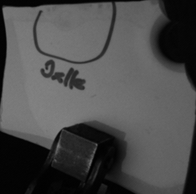
\includegraphics[width = 0.47\textwidth]{04_deflektometrischeRegistrierung/auswertungDeflektometrischeRegistrierung/figures/delleBeleuchtet}
		\caption[Spiegelndes Porzellanbruchstück mit Delle]{Spiegelndes Porzellanbruchstück mit Delle.}
		\label{img:objektMitDelle}
	\end{figure}
}

% Abbildung: Deflektometrische Registrierung bei Objekt mit Delle
{
	\begin{figure}[H]
		\centering
		\begin{adjustbox}{width=\textwidth}
	\begin{tikzpicture}[every node/.style={inner sep=0,outer sep=0}]
	
		\node [anchor=north east] (imgSpalten) at (-0.03\textwidth,0) {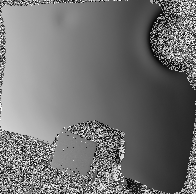
\includegraphics[width=.47\textwidth]{04_deflektometrischeRegistrierung/auswertungDeflektometrischeRegistrierung/figures/spaltenRegistrierung_Delle}};
		\node [below=0.2cm of imgSpalten] {Graubild der Spaltenzuordnung \acrshort{frx}$(x,y)$};
		\node [anchor=north west] (imgZeilen) at (0.03\textwidth,0) {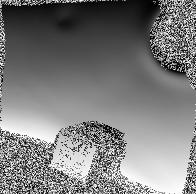
\includegraphics[width=.47\textwidth]{04_deflektometrischeRegistrierung/auswertungDeflektometrischeRegistrierung/figures/zeilenRegistrierung_Delle}};
		\node [below=0.2cm of imgZeilen] {Graubild der Zeilenzuordnung \acrshort{fry}$(x,y)$};
		
	\end{tikzpicture}
\end{adjustbox}
\caption[Deflektometrische Registrierung bei Delle]{Deflektometrische Registrierung des spiegelnden Keramikobjekts aus Abbildung \ref{img:objektMitDelle}.}
		\label{tikz:abbRegistrierungDelle}
	\end{figure}
}

\noindent
In Abbildung \ref{tikz:abbRegistrierungDelle} entsteht im Hintergrund um das Objekt herum eine Störumgebung.
Der Grund dafür ist die fehlende Reflexion des Musters und somit ähnliche Grauwerte in den phasenverschobenen Bildern.
Dies führt dazu, dass in der Bestimmung der Phase $\phi$ für solche Pixel numerisch instabile Ausdrücke und somit schwankende Werte vorkommen.

\p
Die resultierenden Bilder können durch herkömmliche Verfahren aus der Bildverarbeitung weiterverarbeitet und analysiert werden.
Durch die stetigen Grauwertverläufe in den Bildern \acrshort{frx} und \acrshort{fry} an gleichmäßig gekrümmten Oberflächen, lassen sich diese effizient über ihre Ableitungen analysieren (siehe Abbildung \ref{tikz:abbGradientenbildReg}).
Abrupte Änderungen der Grauwerte innerhalb des spiegelnden Objekts führen zu einem höheren Ableitungswert als in der Umgebung. Fehlstellen wie z. B. Dellen oder Pickel lassen sich damit gut detektieren.
Aus demselben Grund erweisen sich auch Hochpassfilterungen als hilfreich \cite{kit_werling}.

% Abbildung: Gradientenbild der deflektometrischen Registrierung.
{
	\begin{figure}[H]
		\centering
		\begin{adjustbox}{width=\textwidth}
	\begin{tikzpicture}[every node/.style={inner sep=0,outer sep=0}]
	
		\node [anchor=north east] (imgSpalten) at (-0.03\textwidth,0) {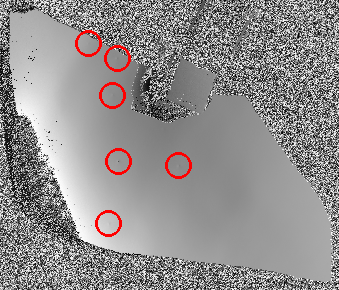
\includegraphics[width=.47\textwidth]{04_deflektometrischeRegistrierung/auswertungDeflektometrischeRegistrierung/figures/pickelDeflektometrischeRegistrierung}};
		\node [below=0.2cm of imgSpalten] {Graubild der Spaltenzuordnung \acrshort{frx}$(x,y)$};
		\node [anchor=north west] (imgGradienten) at (0.03\textwidth,0) {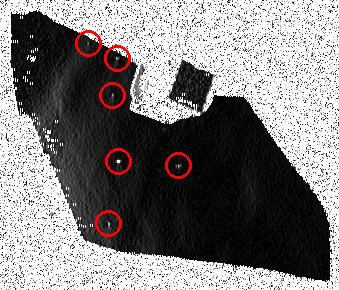
\includegraphics[width=.47\textwidth]{04_deflektometrischeRegistrierung/auswertungDeflektometrischeRegistrierung/figures/pickelGradientenbild}};
		\node [below=0.2cm of imgGradienten, align = center] {Bild der Ableitung von \acrshort{frx}$(x,y)$ \\ in $x$-Richtung};
		
	\end{tikzpicture}
\end{adjustbox}
\caption[Hervorhebung von Pickeln auf reflektierenden Oberflächen.]{Deflektometrische Spaltenregistrierung eines spiegelnden Porzellanbruch\-stücks und das zugehörige Bild der Ableitung. In den rot markierten Stellen lassen sich kleine Abweichungen von einem stetigen Grauwertverlauf erkennen, die in der Ableitung einen Ausschlag haben. Auf dem Prüfobjekt befinden sich an den Stellen kleine Pickel auf der Oberfläche.}
		\label{tikz:abbGradientenbildReg}
	\end{figure}
}

\noindent
Abbildung \ref{tikz:abbGradientenbildReg} zeigt, wie durch die deflektometrische Registrierung kleine Fehlstellen, wie z. B. Pickel auf einer spiegelnden Oberfläche, sichtbar gemacht werden können, die ohne eine spezielle Beleuchtung nicht zu erkennen sind.
Das untersuchte Objekt aus Abbildung \ref{tikz:abbGradientenbildReg} weist am linken Rand vereinzelt matte Stellen auf.
Dadurch treten im Bild der deflektometrischen Registrierung \acrshort{frx} einzelne dunkle Punkte bzw. Artefakte am linken Rand auf.
Diese erkennt man somit auch im Ableitungsbild von \acrshort{frx} als Fehlstellen.

\p
In dem Bild der Ableitung von \acrshort{frx} in $x$-Richtung aus Abbildung \ref{tikz:abbGradientenbildReg} lassen sich Aussagen über die Krümmung der Oberfläche entlang der $x$-Richtung treffen.
Allgemein betrachtet man zu\-nächst eine feste Gerade in der Kameraebene, bezeichnet als Bildkurve.
Die Bildkurve entsteht durch die Spiegelung einer bestimmten Monitorkurve auf einer Oberfläche.
Von der Kurve in der Monitorebene schneiden die ausgehenden Lichtstrahlen die Oberfläche entlang einer Oberflächenkurve.
Über den Zusammenhang der Spiegelabbildung von Geraden und Kurven an gekrümmten Oberflächen lässt sich zeigen, dass die Änderung der Monitorkurve vom linearen Verlauf proportional zur Änderung der Flächennormalen entlang der Oberflächenkurve ist \cite{kit_werling}.
Deutlich wird dies nochmals, wenn man beachtet, dass Geraden bei der Spiegelung nur auf Geraden abgebildet werden können, wenn die Spiegeloberfläche an den Reflexionspunkten einer Ebene entspricht.
Das heißt, dass lokale Änderungen der Tangenten an der Monitorkurve lokalen Abweichungen der Spiegeloberfläche vom ebenen Verlauf entsprechen.
Bekanntlich stellt die deflektometrische Registrierung \acrshort{lr} den Zusammenhang zwischen der Bildebene und der Monitorebene dar.
Demzufolge lässt sich durch das Ableiten der deflektometrischen Registrierung \acrshort{lr} in eine bestimmte Richtung direkt die Abweichung der Flächennormalen, also die wahrgenommene Krümmung der Oberfläche, entlang der Richtung bestimmen.
Die wahrgenommene Krümmung steht in direktem Zusammenhang mit der zweiten Ableitung der Objektoberfläche \cite{kit_werling}.

\p
In Abbildung \ref{tikz:abbGradientenbildReg} erhält man durch die Faltung des Bildes \acrshort{frx} mit Filter für die Ableitung in $x-$-Richtung ein Bild, das in direkter Beziehung zu der Ableitung der deflektometrischen Registrierung \acrshort{lr} in  $x$-Richtung steht.
Somit steht dieses Bild auch im Verhältnis mit der Krümmung der Oberfläche in $x$-Richtung.
Analog lässt sich auch die Krümmung in $y$-Richtung auswerten.

\p
Die deflektometrische Registrierung hat im Vergleich zur Rekonstruktion der Oberfläche essenzielle Vorteile.
Zum Einen kann zur Oberflächenprüfung auf die aufwendige Systemkalibrierung verzichtet werden.
Außerdem ermöglichen die Separierbarkeit und die Darstellung als Bilder den Einsatz von effizienten Methoden aus dem Bereich der Bildverarbeitung.
Das ermöglicht den Einsatz dieser Verfahren für die Erkennung von verschiedenen Fehlstellen auf spiegelnden Oberflächen.
Die Verwendung für transparente Objekte, die Licht durchlassen, ist nur eingeschränkt möglich, da die meiste Information in der Krümmung der Streifenmuster liegt.
Nutzt man also den Monitor als Durchlichtbeleuchtung, ist die Zuordnung trotz vorhandener Fehlstellen überwiegend linear.
Dies kann allerdings auch zum Vorteil genutzt werden, wenn nur diese speziellen Informationen gesucht werden.
}
    }
    
    %Fourier-Streifen-Analyse
    {
    	\FloatBarrier %Verhindert Fehlpositionierung von Abbildungen aus vorherigen Abschnitten
    	\chapter{Fourier-Streifen-Analyse}
    	

    }
    
    %Quellenverzeichnis
    {
    	\FloatBarrier %Verhindert Fehlpositionierung von Abbildungen aus vorherigen Abschnitten
    	\newpage
      \phantomsection
      \addcontentsline{toc}{chapter}{Quellenverzeichnis}
      \printbibliography[title = Quellenverzeichnis]
    }
\end{document}
